\begin{frame}
  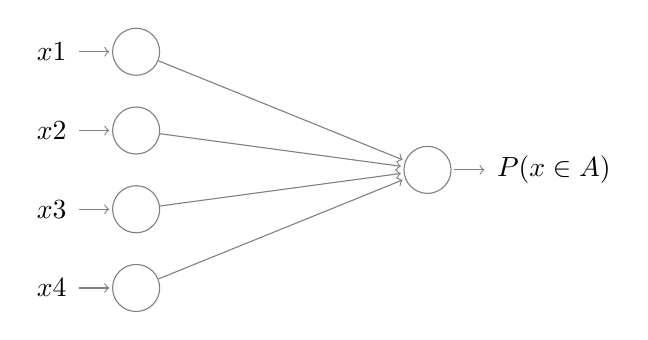
\begin{tikzpicture}[shorten >=1pt,->,draw=black!50, node distance=2.5cm]
    \tikzstyle{every pin edge}=[<-,shorten <=1pt]
    \tikzstyle{neuron}=[circle,draw,minimum size=17pt,inner sep=0pt]

    \foreach \y in {1,2,3,4}
    \node[neuron, pin=left:$x\y$] (I-\y) at (0,-\y) {};

    \node[neuron,pin={[pin edge={->}]right:$P(x \in A)$}, right of=I-3] (O-1) at
    (1.2,-2.5) {};

    \foreach \src in {1,2,3,4}
    \path (I-\src) edge (O-1);
  \end{tikzpicture}
\end{frame}

\begin{frame}
  \begin{tikzpicture}[shorten >=1pt,->,draw=black!50, node distance=2.5cm]
    \tikzstyle{every pin edge}=[<-,shorten <=1pt]
    \tikzstyle{neuron}=[circle,draw,minimum size=17pt,inner sep=0pt]

    % input layer nodes
    \foreach \y in {1,...,4}
    \node[neuron, pin=left:$x\y$] (I-\y) at (0,-\y) {};

    % output layer node
    \path[yshift=-1.4cm]
    node[neuron,pin={[pin edge={->}]right:$P(x \in A)$}] (O-1) at (2.5,0) {};
    \path[yshift=-1.4cm]
    node[neuron,pin={[pin edge={->}]right:$P(x \in B)$}] (O-2) at (2.5,-1) {};
    \path[yshift=-1.4cm]
    node[neuron,pin={[pin edge={->}]right:$P(x \in C)$}] (O-3) at (2.5,-2) {};

    % Connect every node in the input layer with every node in the
    % output layer.
    \foreach \src in {1,...,4}
    \foreach \dst in {1,2,3}
    \ifthenelse{\equal{\dst}{1}}
    {\path[draw=red] (I-\src) edge (O-\dst)}
    {\path[draw=black!50] (I-\src) edge (O-\dst)};
  \end{tikzpicture}
\end{frame}
